% lit. survey II
The description of unbound particles has several complications of conceptual and technical kind.
%Some methods to obtain the FEF had been mentioned in section \ref{ch:r-mat} already, 
In this chapter, different numerical methods are introduced that can be used to solve the one-electron SE.
In section \ref{ch:contwa}, the conceptual differences between bound and continuum states as well as the numerical treatment of the latter in a finite basis are discussed.
Thereafter, in the sections \ref{ch:FD} - \ref{ch:wavelet}, different numerical methods are introduced that can be used to solve the one-particle SE on a molecular domain.
%These methods can be roughly divided into two main classes: In section \ref{ch:FD} the finite difference and finite volume methods are introduces which both are based on the approximation of the operators by differences of function values.
%The other methods are based on different basis expansions wich are designed with different properties
%\textcolor{red}{Need to think a bit how to expand on this. Moreover: splines don't fit in there, do they? --> need further category?}
% based on finite differences, a basis-expansion of finite element.

\section{Continuum Waves}
\label{ch:contwa}
Continuum waves are discussed only sparsely in lectures on quantum mechanics, even though they posses certain fundamental differences compared to bound states.
The states considered here have a spacially infinite extend as it is well-known for plane waves 
\begin{equation}\label{eq:PlWave}
\Psi^\text{plan}(\vec{r})=\sqrt{\frac{|\vec{k}|}{(2\pi)^3}}e^{i\vec{kr}}
\end{equation}
with wave-vector $\vec{k}$ as well as for spherical waves. %whose radial part contains different powers of $\frac{\sin(kr)}{kr}$ \cite{Lifschitz}.
Moreover, these waves are not square integrable and hence can not be normalised according to $\int \Psi^\dagger(\vec{r})\Psi(\vec{r}) d\vec{r}=1$ and thus the probability interpretation is invalid \cite{quirky}.
Instead, these functions are sharp in a continuous variable (namely the momentum) and hence should rather be interpreted as probability densities, suggesting the normalisation 
$\int \Psi^\dagger(\vec{r})\Psi(\vec{r'}) d\vec{r}=\delta(\vec{k}-\vec{k'})$ where $\delta(\vec{k})$ is the Dirac delta distribution \cite{quirky}.
This property distinguishes the analytical FEF from those obtained with numerical methods that often have a finite extent and are obtained from an approximate Hamiltonian matrix which has no continuous spectrum due to finiteness of its basis.
Especially the difference in the normalisation of wave functions and by this in the dimensionality of overlap integrals also affects the integral evaluated when calculating the transition dipole matrix elements \cite{stieltjesCeder}.
However, the Stieltjes imaging approach described in section \ref{ch:stieltjes} gives a formal varification for the use of square-integrable function for the representation of a continuum state. %since it can be considered as $0$-th order moment expansion.
Moreover, it provides a formalism to enhance the quality of spectra obtained with numerical methods.

A further aspect of numerical treatment of continuum functions that is only sparsely discussed in literature concerns the question of the physical interpretation of the numerical solution.
When dealing with approximate continuum functions, it is often assumed that the analytic function of interest $|\Psi_\text{a}(\vec{k})\rangle$ is approximated by that particular numeric solution $|\Psi_\text{n}(\vec{k}')\rangle$ which is closest in energy to the desired one \cite{H2pDeCleva}.
An alternative interpretation would be to assume that the numerical solution corresponds to an approximation to $|\Psi_\text{n}\rangle \approx \frac{1}{k^+-k^-} \int_{k^-}^{k^+}|\Psi_\text{a}(k) \rangle dk$ which would change the interpretation and normalisation.
%
%This rises the question, whether a numerically obtained free electron state corresponds most to the analytic state with the same kinetic energy, hence
%$\Psi\approx \Psi_k$
%or whether it should be considered more as an integration over a small part of the spectrum
%$\Psi\approx \frac{1}{k^+-k^-} \int_{k^-}^{k^+}\Psi(k) dk$
%which changes the interpretation and normalisation required for the wave function.

In other works simulating PES in frequency domain, mainly two different representations of the photoelectron are found which are based on plane-wave expansions in spherically symmetric bases \cite{ezDyson,DO_TDDFT,do_modCoul}.
One of the expansions is that in spherical waves \cite{Lifschitz}
\begin{equation} \label{eq:spherWave}
\Psi^\text{Sph}_{\vec{k}}(\vec{r})=4\pi
\sum_{l=0}^\infty \sum_{m=-l}^l \text{i}^l j_l\left(kr\right), Y_l^m\left(\theta, \phi\right) Y^{\dagger,m}_l\left(\theta_k, \phi_k\right)
\end{equation}
where $k=|\vec{k}|$ is the length of the wave vector $\vec{k}$, $j_l(kr)$ are spherical Bessel functions that solve the radial SE (eq. (\ref{eq:radSEeq}) with $V(r)=0$) and the arguments to the spherical Harmonics $Y_l^m$, $(\theta,\phi)$ and $(\theta_k,\phi_k)$, are the angles of the spherical coordinate system in real-space and Fourier-space, respectively \cite{ezDyson}.
Another expansion of a plane wave often used that in Coulomb waves
\begin{multline} \label{eq:CoulWave}
\Psi^\text{Coul}_{\vec{k}}(\vec{r})=\frac{1}{(2\pi)^{\frac{3}{2}}}
\sum_{l=0}^\infty \sum_{m=-l}^l \text{i}^l (2kr)^l e^{-\pi\frac{Z}{2k}} \frac{|\Gamma(l+1+i\frac{Z}{k})|}{\Gamma(2l+2)} \\
e^{ikr} F_1(l+1-i\frac{Z}{k}, 2l+2, 2ikr) 
Y_l^m\left(\theta, \phi\right) Y^{\dagger m}_l\left(\theta_k, \phi_k\right)
\end{multline}
where $Z$ is the change of the nucleus and $F_1$ is the confluent hypergeometric function of the first kind \cite{do_modCoul,ColWave} \footnote{$F_1(\alpha,\gamma,z)=1+\frac{\alpha}{\gamma}z + \frac{\alpha (\alpha+1)}{\gamma (\gamma+1)} \frac{z^2}{2!}+\hdots $}.
Assuming $Z=-1$, \textit{i.e.} the case of the hydrogen atom, the limit $k\rightarrow 0$ the confluent hypergeometric function is
\begin{equation}
\lim_{k\rightarrow 0} F_1(l+1+\frac{i}{k}, 2l+2, 2ikr) =(2l+1)! (2r)^{-l-\frac 12} J_{2l+1}(\sqrt{8r})
\end{equation}
where $J_{2l+2}(x)$ is the Bessel function that is connected with the spherical Bessel functions $j_l(x)$ via the relation $j_l(x)=\sqrt{\frac{\pi}{2x}} J_{l+\frac 12}(x)$ \cite{Lifschitz}.
This case is separately available in \prog{ezDyson} \cite{ezDyson}.

The latter approach accounts for the electrostatic potential of the remaining anion at larger distances to the molecule but does not account for the Coulomb singularities due to the particular molecular structure respectively.
To correct for this error which becomes significant especially for lower kinetic energies where the influence of the potential is stronger, \textit{e.g.} an effective charge $Z^*<1$ is used \cite{do_modCoul} or the ansatz function is orthonormalised with respect to the DO \cite{do_orthonorm,do_orthonorm1,do_pworth} which can be shown to be equivalent to a respective shift of the coordinate system such that the expectation value of the dipole moment of the DO vanishes \cite{do_orthonorm}.

\begin{figure}
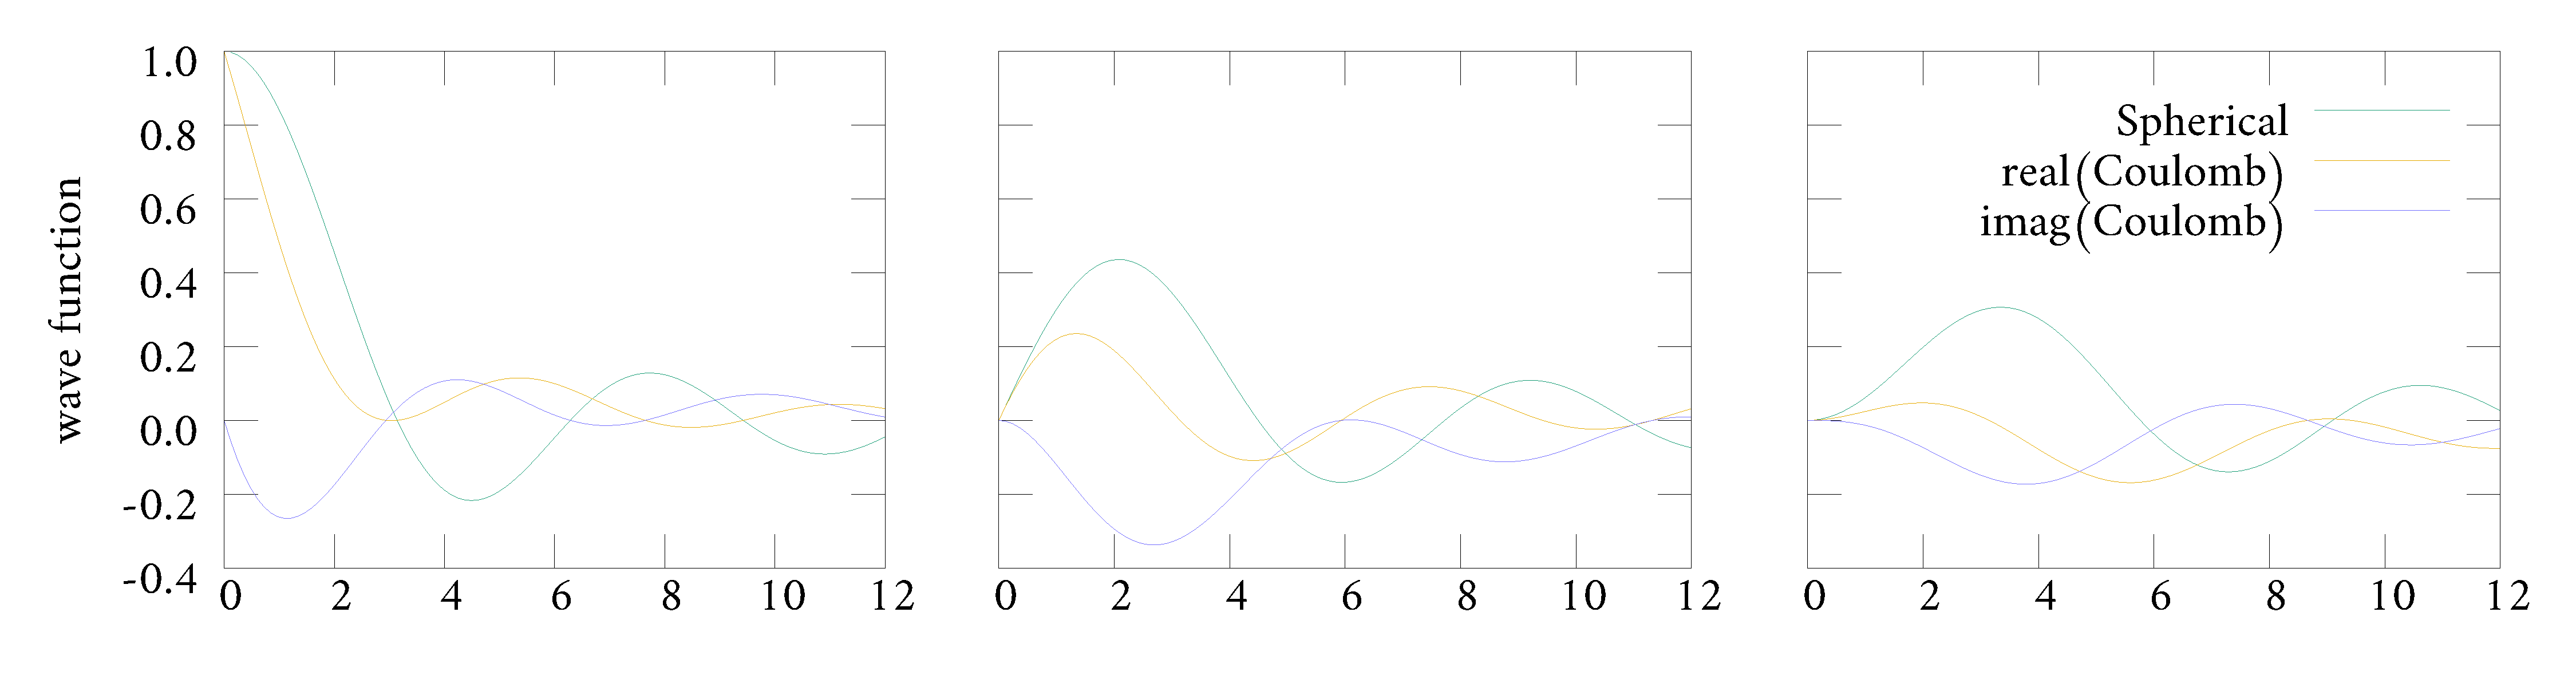
\includegraphics[width=\textwidth]{Figures/RBF/RadialPart}
\caption{Radial part of spherical waves and Coulompart of spherical waves and Coulompart of spherical waves and Coulompart of spherical waves and Coulompart of spherical waves and Coulompart of spherical waves and Coulompart of spherical waves and Coulompart of spherical waves and Coulompart of spherical waves and Coulomb waves (confluent hypergeometric function approximated with 35 terms each) for $l=0$ (left), $l=1$ (centre) and $l=2$ (right).
The Coulomb waves are not normalised respectively.}
\label{fig:RadFun}
\end{figure}
The spherical Harmonics moreover have the form
\begin{equation}\label{eq:SphHarm}
Y_l^m(\theta,\phi)= (-1)^{(m+|m|)/2} i^l \sqrt{\frac{2l+1}{4\pi}\frac{(l-|m|)!}{(l+|m|)!}}  P_l^{|m|}(\cos(\theta)) e^{im\phi}
\end{equation}
where $P_l^m(x)$ are associated Legendre polynomials \cite{Lifschitz}.
The spherical harmonics are orthonormal with respect to the indices $l$ and $m$.

In this work the spherical waves (\ref{eq:spherWave}) are used as reference basis for the computed solutions for an easier interpretation and comparison of different results.

Another conceptual question is about the infinite degeneracy of the analytic solution which becomes clear when considering an example of the ionisation of a hydrogen-like atom whose analytical FEF is well-known and has the form \cite{Lifschitz}
%
%In addition to the transition from a continuous to a discontinuous spectrum, also degerarcy plays an important role.
%This can be best discussed when taking the example of the ionisation process of a hydrogen atom where the corresponding FEF has the analytic form

The function (\ref{eq:CoulWave}) is, given its energy $E=\frac 12 |\vec{k}|^2$, infinitely degenerate in the direction of $\vec{k}$ as well as in the quantum numbers $l$ and $m$.
Hence the wave function of a photoelectron can consist of any superposition of the form (\ref{eq:CoulWave}), chosing the coffecients $c_{l,m}$ accordingly.
The coefficients $c_{l,m}$ of the physically observable FEF are determined by the matrix elements of the dipole operator with the DO (\ref{eq:sigma_do}).  
Considering as an example the ionisation of hydrogen in its ground state, the FEF is in one of the three $p$-waves because the probability to access any of the other vaccum-states with the correct energy vanishes due to dipole selection rules for spherically symmetric systems.

Unfortunately, as will be shown below in section \ref{ch:resBench}, the considerations made above are not true for the numerical solution anymore where a finite set of superpositions is obtaind which, due to numerical treatment, differ in energy and thus can not be assigned to a common value of $\vec{k}$.
Chosing the energetically best-fitting solution though might in principle result in a function with vanishing contribution of the $p$-type orbitals while, for slightly changed computational schem or target energy could yield a solution with large $p-$contributions with.

%The coefficients $c_{l,m}$ moreover are arbitrary coefficients to this end since any of the linear combinations solves the SE for a given kinetic energy.
%Hence analytical the solutions are not only continuous in $\vec{k}$, but also infinitely degenerate in $l$ and $m$.
%In contrast to this, the numerical solution will be a linear combination of some of these terms; in the easiest case it is close to one of these $l$ and $m$.
%However, for the case of ionisation from the hydrogen ground state only the contributions with $l=1$ will lead to a transition probability; having a solution of $l=2$-character would lead to vanishing probability.
%Hence, the lifting of degeneracy would lead to intensities that are very sensitive to the kinetic energy of the photoelectron since the $l=1$ solution might be only few meV off that solution of $l=2$-type.
%Moreover, the numerical grid may influence this dependency since it could, by accident, supporting certain symmetries.
%
%A detailed discussion of the conceptual complications arising from this is not found in the literature.
%The FEF used to describe the ionisation of H$_2$ as discussed in \cite{H2pDeCleva} is chosen as that function which fits the target energy best.
%However, in their formulation this energy is well-separated from the others % (spline base without boundary conditions, leading to non-hermitian Hamiltonian). -> do they implicitly use some boundary conditions ?
%They also discuss formulation as minimisation problem: More stable but they don't need it.
%which will be later shown to be not the case here.

\subsection{Stieltjes Imaging}
\label{ch:stieltjes}
The Stieltjes imaging provides an elegant way to still use the numerially obtained solutions of a non-continuous spectrum by using moment theory.
Starting from the expression for the photoelectron spectrum 
\begin{equation}
\sigma(\varepsilon)\propto \left|\langle \Psi_0 |\hat{d}|\Psi_\text{el} \rangle \right|^2
\end{equation}
where $\Psi_\text{el}$ is a continuum function and as such, as discussed above, not square integrable which is an important characteristic for the dimensionality of this expression \cite{stieltjesCeder}.
To repair this, the Stieltjes imaging approach uses spectral moments, where  the $n$-th spectral moment is of the form
\begin{equation}
   M_n=\langle \Psi_0 |\hat{d} (\hat{H}-E_0)^n \hat{d} | \Psi_0  \rangle
\end{equation}
where $\hat{H}$ is the systems Hamiltonian and $E_0$ is the ground state energy \cite{langhoff3}.
Inserting the closure relation $\sum_\alpha |\Psi_\alpha\rangle\langle \Psi_\alpha|+\int |\Psi_\varepsilon\rangle\langle \Psi_\varepsilon| d\varepsilon$ for the full (anatlytic) Hamiltonian results in
\begin{align}\label{eq:M_n_ana}
   M_n&=\sum_\alpha \langle \Psi_0 |\hat{d} (\hat{H}-E_0)^n|\Psi_\alpha\rangle\langle \Psi_\alpha| \hat{d} | \Psi_0  \rangle
      + \int  \langle \Psi_0|\hat{d} (\hat{H}-E_0)^n|\Psi_\varepsilon\rangle\langle \Psi_\varepsilon| \hat{d} | \Psi_0  \rangle d\varepsilon \\
      &= \sum_\alpha \left(E_\alpha-E_0\right)^n \left|\langle \Psi_0 | \hat{d}| \Psi_\alpha\rangle \right|^2 + 
         \int_{0}^\infty \varepsilon^n \left|\langle \Psi_0 | \hat{d}| \Psi_\varepsilon\rangle \right|^2 d \varepsilon.
\end{align}
However, inserting the unity expression for the numerical Hamiltonian which does not have continuum functions but an everywhere discrete spectrum and hence $L^2$-integrable eigenfunctions results in
\begin{equation} \label{eq:M_n_num}
      M_n= \sum_{j=0}^N (E_j-E_0) \left| \langle \Psi_0 | \hat{d}| \Psi_j\rangle \right|^2
\end{equation}
where $N$ denotes the number of eigenfunctions $|\Psi_j\rangle$ \cite{stieltjeLanczos,stieltjesCeder}.
For a good numerical approximation, the expressions (\ref{eq:M_n_num}) and (\ref{eq:M_n_ana}) should be similar for as many $n$ as possible where, due to convergence of the spectral moments, $n<2$ \cite{stieltjesCeder}.
These considerations are used in the Stieltjes imaging approach with moment theory \cite{langhoff, langhoff2}.

In the protocol derived from this scheme thus the oscillator strength $|\langle \Psi_0|\hat{d}|\Psi_\text{el}\rangle|^2$ is approximated by the histogram
\begin{equation}
\sigma(\varepsilon)=\frac 23 \frac{df}{d\varepsilon}
      =\frac 23 \begin{cases} 0 & 0< \varepsilon <\varepsilon_1(n) \\
      \frac 12 \frac{(f_i+f_{i+1})}{\varepsilon_{i+1}-\varepsilon_i}  & \varepsilon_j(n)<\varepsilon<\varepsilon_{j+1}(n)\\
      0   & \varepsilon_n(n)<\varepsilon \end{cases}
\end{equation}
%where $f_i$ is obtained from enforcing the relation (\ref{eq:M_n_num}) for $n=1,\hdots, m$ which is done by solving the matrix equation
where $(\varepsilon_i,f_i)_{i=1,...,l}$ are the principal pseudo spectra \cite{stieltjeLanczos} that are obtained from

\begin{equation} \label{eq:StieltMat}
   \vec{M}=\mat{E}\vec{f}
\end{equation}
where $\vec{f}_i=f_i$, $\vec{M}_i=M_i$ and $\mat{E}_{i,j}=\varepsilon_i^j$ \cite{langhoff3}.
It can be shown moreover that $M_n$ is only for $n<2$ finite and therefore negative moments are used \cite{stieltjesCeder}.
Moreover, it can be shown that the expression (\ref{eq:M_n_num}) converges already for small $N$, so only a small fraction of the spectrum needs to be considered in practice and the matrix equation (\ref{eq:StieltMat}) remains at a reasonable size. 
Usually not more than $10-12$ moments are used to avoid spurious oscillations due to unconverged high order moments \cite{stieltje}.

In practice this method becomes very demanding if energetically narrow transitions occur since many terms in expression (\ref{eq:M_n_num}) are needed for convergence, making this method effective mainly for low energy range \cite{H2pDeCleva}.
Another disadvantage that no asymtotic information about this scheme present \cite{H2pDeCleva}.

\section{Finite Differences and Finite Volumes}
\label{ch:FD}
The most common and straightforward approach to solve differential equations numerically is via the so-called finite difference (FD) scheme.
Starting from the one-particle SE in atomic units
\begin{equation} 
\left( \frac 12 \nabla^2 + V(\vec{r}) \right) \Psi(\vec{r})=E\Psi(\vec{r})
\end{equation}
where $V(\vec{r})$ is an arbitrary potential at this point.
Considering a general problem where the low symmetry does not support a product ansatz which would reduce the dimensionality and thus the complexity of the problem, the kinetic energy operator has at least $6$ non-diagonal terms which lead to an Hamiltonian of a non-banded structure \cite{fd_Cart}.
Moreover, the finite-difference schemes require the evaluation points to be on a regular grid whose size is governed by the sharpest features in the system while local refinement is hardly available.
To resemble the expected fine structure close to the nuclei, a dense grid is needed but any FD scheme beyond the first order requires the evaluation points to be on a regular grid, making the computation of a FEF with a reasonable box size very expensive \cite{richardsFD}.
Nonetheless, there are applications to this scheme to the SE \cite{fd_Cart,fd_Cart2}, some of them with massive parallelisation using MPI and multiple GPUs \cite{fd_gpu}.

To overcome this bottleneck for systems with non-uniform parameters, often the finite volume method is used.
The finite volume method is an integral method that is not based on a regular grid.
Instead, for the estimation of the kinetic energy Gau\ss's theorem $\int_V \nabla \vec{u}(\vec{r}) dV=\int_{\partial V} \vec{u}(\vec{r}) \vec{n}dS $ is used where $\vec{u}(\vec{r})$ is a vector-valued function and $\vec{n}$ is the normal vector on the surface $S$ of the volume $V$ under consideration.
Chosing $\vec{u}(\vec{r})=\nabla\Psi(\vec{r})$ yields the relation
\begin{equation} \label{eq:kinFV}
   \nabla^2\Psi(\vec{r})=\lim_{V\rightarrow 0} \frac{ \int_{\partial V} \nabla\Psi(\vec{r}) \vec{n} dS}{V}.
\end{equation}
This scheme becomes especially interesting when the finite volume elements are chosen to be Voronoi cells \cite{Son_Chu0}.
A Voronoi-tesselation is associated with a grid and is constructed such that the Voronoi cell $T_i$ consists of all points in space that are closer to the point $i$ than to any other points in the grid \cite{voronoi,voronoi1,voronoi2}.

This description has the advantage that the quantities on the right-hand side of (\ref{eq:kinFV}) can be associated with properties of the Voronoi-Cell, leading to the first-order approximation of the kinetic energy
\begin{wrapfigure}{l}{0.5\textwidth}
   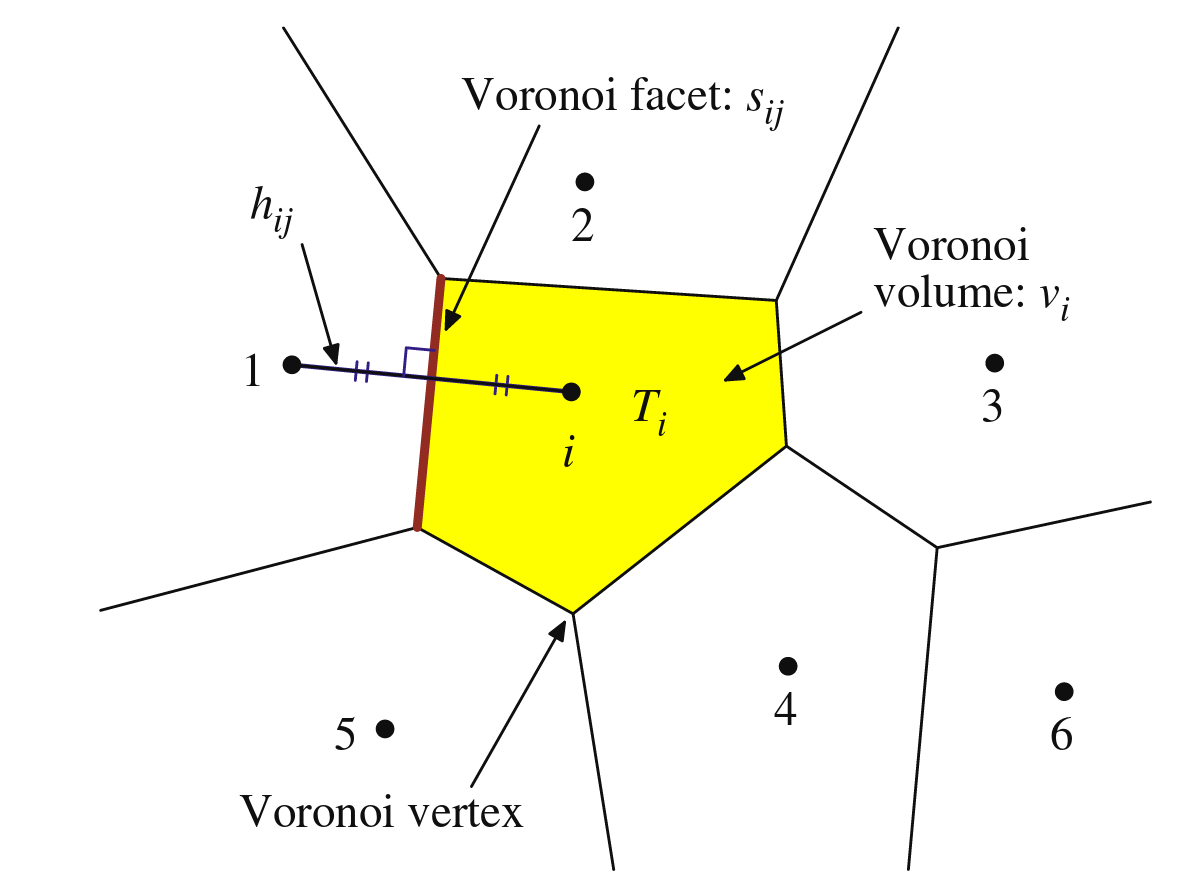
\includegraphics[width=0.5\textwidth]{Figures/VoronoiFD}
   \caption{2-dimensional Voronoi diagram on an arbitrary point-distribution. \cite{Son_Chu}}
   \label{fig:VorCell}
\end{wrapfigure}
\begin{equation}\label{eq:kinVoron}
   \nabla^2\Phi(\vec{r}_i)=\frac{1}{v_i} \sum_j^\text{neighbours} \frac{\Psi(\vec{r}_j)-\Psi(\vec{r}_i)}{h_{ij}} s_{ij}a
\end{equation}
where $v_i$ is the volume of the $i$-th Voronoi-cell, $h_{ij}=|\vec{r}_i-\vec{r}_j|$ is the distance between the centres of the $i$-th and $j$-th Voronoi-cell and $s_{ij}$ is the lengthe of the common facet of the $i$-th and $j$-th Voronoi cell.

Such a scheme is applied \textit{e.g.} by Son and Chu \cite{Son_Chu0, Son_Chu} to the time-dependent SE, studying multi-photon ionisation of several molecular systems.

%\section{Discrete Variable Representation and Splines}
\section{Pseudospectral Methods}
\label{ch:dvr}
Under the term (pse)udospectral methods a large group of methods is comprised which treat the differential equation of interest variationally using an orthogonal basis $span\{\varphi_i(\vec{r})\}$, hence seeking for a solution of the form
\begin{equation}
\Psi(\vec{r})=\sum_i^n c_i \varphi_i(\vec{r})
\end{equation}
where $c_i$ are coefficients to be found \cite{SpectMeth}.
In the pseudospectral methods the basis functions $\varphi_i(\vec{r})$ are smooth global functions such as $\varphi_{\vec{k}}(\vec{r})=\frac{1}{(2\pi)^\frac 32 }e^{\text{i}\vec{k}\vec{r}}$ resulting in the Fourier method \cite{Fourier}.
Alternatively Jacobi, Chebychef or Legendre polynomials are commonly used \cite{PSbook}.

To find the corresponding coefficients, the equation is evaluated on a grid, leading to a linear system of equations to be solved.
Depending on the technique used for determining the coefficients, it can be seen as a high-order FD or high-order ($p$-) finite element method (FEM).
One large advantage of this class of methods is that the error of the solution $\psi(\vec{r})$ usually decays exponentially with the number $n$ of basis functions and the grid can be chosen coarsely, making the numerical scheme very efficient \cite{PSbook, Tannor}.
In addition, many formulations allow for an implementation making use of the fast fourier transform \cite{PSbook}.

A special representative subgroup of the pseudospectral methods are the so-called discrete variable representation (DVR) schemes which are frequencly used to study quantum chemical problems \cite{yipDVR,impLDVR,coulDVR}.
Since this scheme is applicable in one dimension only, often symmetry-adapted coordinates such as spherical coordinates are used and the ansatz
\begin{equation}
  \varphi= \sum_{l, m} R_{l,m}(r) Y_l^m(\theta, \phi)
\end{equation}
is applied where $Y_l^m(\theta, \phi)$ are the well-known spherical harmonics \cite{SphHarm} and $R_{l,m}(r)$ are radial functions that are computed explicitly, solving the radial SE.

The basis functions used in this scheme commonly are Lagrange polynomials \cite{taoDVR,impLDVR,coulDVR} whose nodes are chosen by a general Gau\ss quadrature rule \cite{impLDVR} or from a quadrature rule for the radial Coulomb function which is in particular popular for quntum chemical problems \cite{coulDVR,Tannor}.
Even if the DVR provides a flexible and fast-convergent basis, an extension to higher dimensionality can be achieved by a product ansatz only and thus is applicable to problems with high symmetry only.

Moreover, as for the other pseudospectral methods, the system matrices are dense and thus the solution is numerically expensive.
This is, at least in parts, solved by using a hybrid scheme of the finite element and DVR scheme where the DVR scheme is used on small segment only, connected by single bridge-functions each \cite{taoDVR,impLDVR}.

\section{Radial Basis Functions}
The radial basis function (RBF) technique is a basis that is based on an arbitrary point distribution with very general properties.
The basis functions $\varphi_i(\vec{r})$ used in this technique need to be spherically symmetric, \textit{i.e.} $\varphi_i(\vec{r})=\varphi_i(|\vec{r}|)$ and are placed at the grid points of a given domain.
Among the commonly used functions are, besides linear and cubic functions, multiquadratic ($\sqrt { r^2 + r0^2 }$), inverse multiquadratic ($\frac{1}{ \sqrt { r^2 + r0^2}}$) and Gaussian ($ e^{-\frac{r^2}{2r_0^2}}$) functions \cite{rbfSE,rbfWave}.

If the parameter $r_0$ is chosen reasonably the scheme is numerically stable and fast-convergeing \cite{rbfSE}.
Another advantage is the straight-forward implementation and generality of this method.
But the coise of $r_0$ can be non-trivial especially for highly non-regular grids where the occurring large distances require broad and smooth functions which lead to instabilities for close-lying points.
Moreover the resulting system matrices are dense due to the global definition of the ansatz functions, making it compputationally expensive.
\begin{wrapfigure}{r}{0.6\textwidth}
   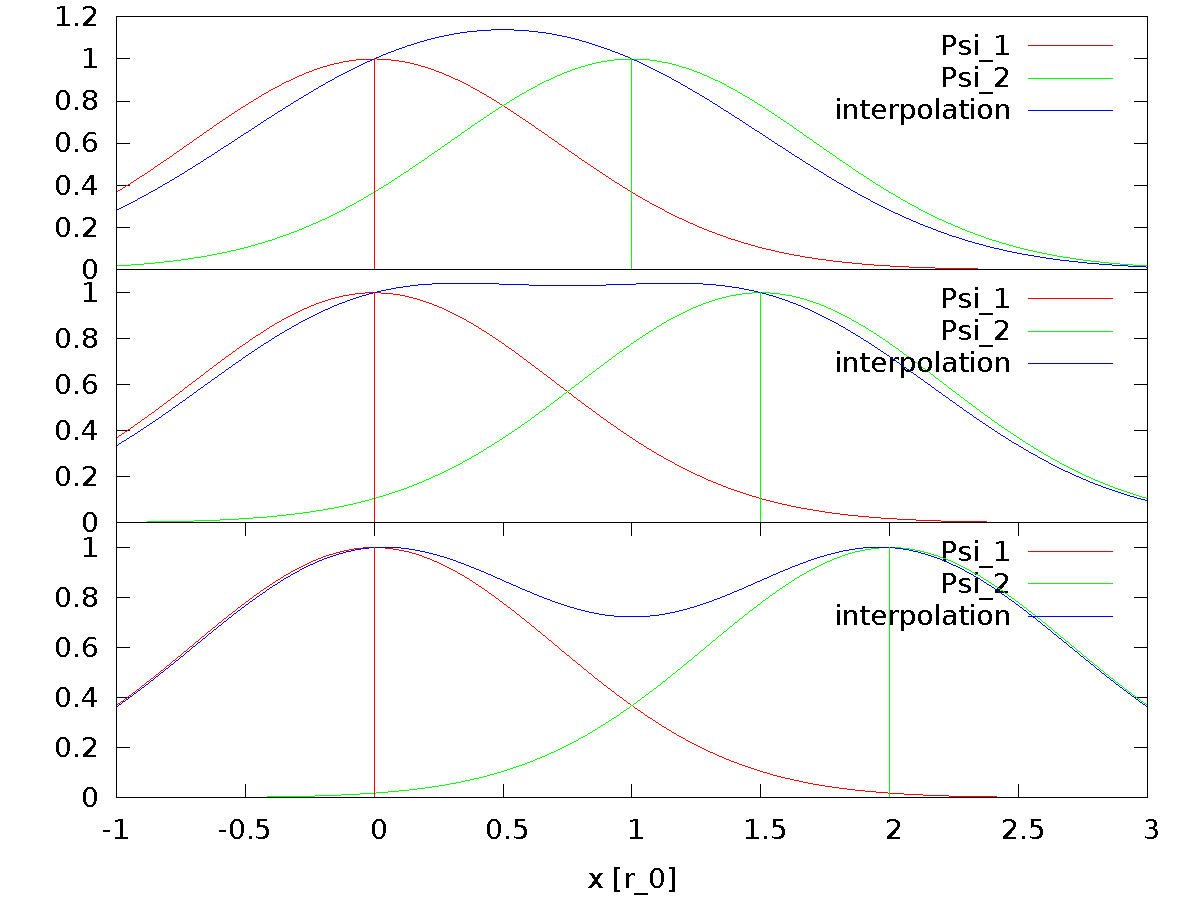
\includegraphics[width=0.6\textwidth]{Figures/RBF/RBFerror}
   \caption{A function (blue) represented in a RBF basis with Gaussian functions, centred at different distances compared to the broadening parameter $r_0$.}
   \label{fig:rbfError}
\end{wrapfigure}

The RBF-scheme is used not only for solving differential equations but is also a usefull tool for interpolation of scattered data in arbitrary dimensions \cite{rbfInterpol} and surface reconstruction from scattered data \cite{rbfSurf}.

An important disadvantage of the RBF scheme is that the space between two interpolation points is interpolated non-linearly and, depending on the distance of the two functions, the values are over- or underestimated.
This error is visualised in Figure \ref{fig:rbfError} for the case of a function that is one at both supporting points, represented by a Gaussian RBF basis.
The intermediate course of the function depends strongly on the ratio of the broadening $r_0$ and the difference between the supporting points.

While this behaviour is not problematic for visual purposes, it may introduce a substructure which can lead to unintended behaviour of the solution.
Since on irregular grids strongly varying distances between supporting points occur, this behaviour is stronger the less regular the initial data are.

\section{Finite Elements}
\label{ch:introFEM}
In the FEM the differential equations to be solved are formulated in their weak form that can be understood as a generalisation of it.
Starting with the well-known (strong) form of the SE defined on a domain $ \Gamma$ in atomic units which are used here and in the following chapters
\begin{equation} \label{eq:SEstrong}
-\frac 12 \nabla^2\Psi(\vec{r})+ V(\vec{r})\Psi(\vec{r})=E \Psi(\vec{r}) \qquad  \vec{r}\in \Gamma
\end{equation}
with the condition for the boundary domain $\partial \Gamma$ which is assumed to be Lipschitz continuous
\begin{equation}
    %\lim_{\vec{r}\longrightarrow \infty} \Psi(\vec{r})=0
    \Psi(\vec{r})=0  \qquad \vec{r} \in \partial \Gamma.
\end{equation}
The first term in equation (\ref{eq:SEstrong}) corresponds to the kinetic energy and $V(\vec{r})$ is a potential that is not further specified at this point.
The unknowns of this equation are the wave function $\Psi(\vec{r})$ and respective energy $E$.
To bring equation (\ref{eq:SEstrong}) into the weak form, it is first multiplied by the complex conjugate of a test function $\Phi(\vec{r})$ which fulfils the same boundary conditions and needs to be differentiable.
In the second step, one integrates over the whole space of interest resulting in
\begin{align}
\int d \vec{r} & \left( - \frac 12 \left(\nabla^2\Phi^*(\vec{r})\right)\Psi(\vec{r})
               + V(r) \Phi^*(\vec{r}) \Psi(\vec{r})\right) = E \int d \vec{r} \Phi^*(\vec{r}) \Psi(\vec{r}).
\end{align}
The kinetic energy term can be symmetrised using Green's first identity $\int_\Gamma (\nabla^2\Psi)\Phi^* d\vec{r}=\int_{\partial \Gamma} (\nabla\Psi)\Phi^* ds -\int_\Gamma (\nabla\Psi)(\nabla\Phi^*)$ to obtain the final expression
\begin{align}\label{eq:SEweak}
\int d \vec{r} & \left(  \frac 12 \left(\nabla\Phi^*(\vec{r})\right) \left(\nabla\Psi(\vec{r})\right) 
               + V(r) \Phi^*(\vec{r}) \Psi(\vec{r})\right) = E \int d \vec{r} \Phi^*(\vec{r}) \Psi(\vec{r})\\
   % &\lim_{\vec{r}\longrightarrow \infty} \Phi(\vec{r})=0.\qquad
   % \lim_{\vec{r}\longrightarrow \infty} \Psi(\vec{r})=0.
    &\Phi(\vec{r})=0\quad
     \Psi(\vec{r})=0\quad  \vec{r}\in\Gamma
\end{align}
which is denoted as the weak form of the SE.
A function $\Psi(\vec{r})$ is considered as a solution of (\ref{eq:SEweak}) if the equation holds for any test function $\Phi(\vec{r})$.
Since usually only real-valued bases functions are used, in the literature the complex conjugation is omitted.
From a mathematical point of view, since $\Phi(\vec{r})$ is an arbitrary function, complex conjugation does not change anything here but it will be shown later that it is more reasonable from a physical point of view if the weak formulation is defined as given in equation (\ref{eq:SEweak}).

The weak formulation (\ref{eq:SEweak}) has two main differences compared to the strong formulation (\ref{eq:SEstrong}).
The first is that any solution of (\ref{eq:SEstrong}) solves (\ref{eq:SEweak}) while the space of solutions of the weak form is larger since only first derivatives need to be defined, which lead to the terms weak and strong respectively.
In addition, a weak solution is defined only up to a cardinal number of zero; hence changing the values of a given solution $\Psi(\vec{r})$ along a finite number of planes in three dimensions yields a function that still solves (\ref{eq:SEweak}).
These properties play an important role here since they allow \textit{e.g.} for piecewise linear basis functions as they are commonly used in the FEM scheme which do not have a second derivative and whose first derivative is undefined on areas with a cardinal number of zero.

To obtain the finite element formulation, one does not work on the whole space of differentiable and quadratically integrable functions defined on $\Gamma$ but restricts the space to subspace spanned by a finite set of test functions for both $\Psi(\vec{r})$ and $\Phi(\vec{r})$, leading to the Petrov-Galerkin scheme.
To get best flexibility for the wave function, the domain $\Gamma$ is subdivided into finite volume elements with a close packing.
These volume elements, denoted as finite elements, give this method its name.
Having this subdivision of space, the ansatz (basis) functions $\varphi(\vec{r})$ used to construct $\Psi(\vec{r})$ and $\Phi(\vec{r})$ are defined as piecewise polynomials being non-zero only on one or few elements.\\
Considering $\Gamma$ to describe a plane, the elements can be for example triangles as shown in Figure \ref{fig:2Del}.
In this plane the vertices of the triangles can be enumerated as $\vec{r}_i\, i=1,\hdots ,N $, leading to the definition of piecewise linear basis functions
\begin{equation}\label{eq:femAnsatz}
   \varphi_i(\vec{r}_j)=
           \begin{cases} 1  & j=i \\
                         0  & j\neq i \end{cases}
\end{equation}
resulting it two dimensional ``hat'' functions as depicted in Figure \ref{fig:2Del}.
\begin{wrapfigure}{r}{0.75\textwidth}
   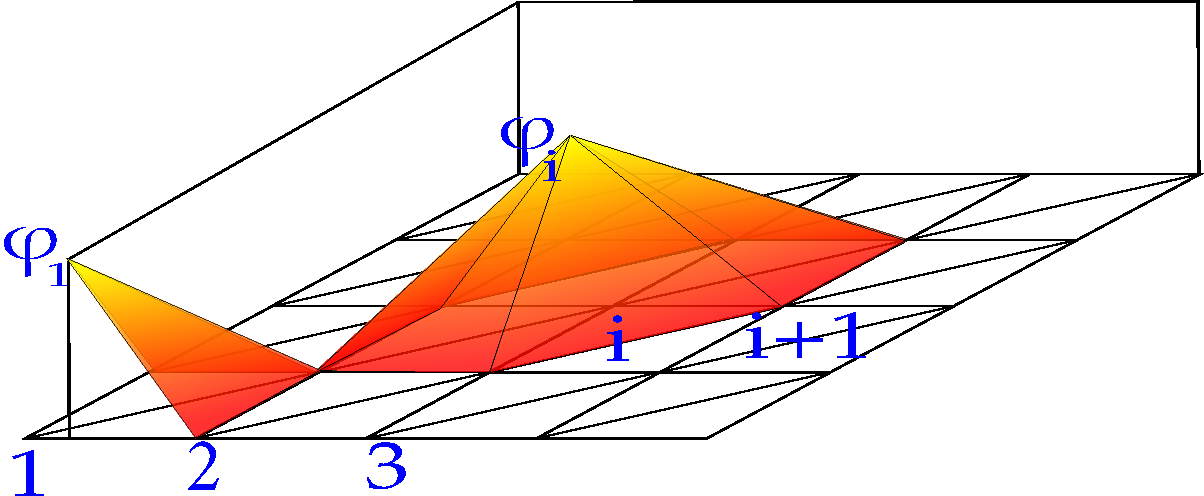
\includegraphics[width=.75\textwidth]{Figures/FEM2d-crop}
   \caption{Example of finite elements in 2D of triangular shape and linear basis functions $\varphi_i(\vec{r})$ defined on them.}
   \label{fig:2Del}
\end{wrapfigure}
The so defined basis ensures continuity of the solution over $\Gamma$ while the first derivatives are continuous only within each element.
To assure continuity of the first derivatives as well, second order polynomials are needed.

As usual in variational schemes, the wave function of interest is a linear combination of these basis functions $\Psi(\vec{r})=\sum_i c_i \varphi_i(\vec{r})$ where $c_i$ are weighting coefficients.
The test functions are chosen from the same space of ansatz functions, testing each basis separately $\Phi(\vec{r})=\varphi_j(\vec{r}), j\in {1,\hdots, N}$.
Hence, the SE (\ref{eq:SEweak}) is rewritten as
\begin{multline}
     \sum_i \int d  \vec{r} \left(\frac 12 \left(\nabla\varphi_i(\vec{r})\right) \left(\nabla\varphi_j(\vec{r})\right) +
                             V(r) \varphi_i(\vec{r}) \varphi_j(\vec{r}) \right) c_i =
               E \sum_i \int d \vec{r} \varphi_i(\vec{r}) \varphi_j(\vec{r}) c_i \\
                      \quad \forall j \in \{1,\hdots ,N\}
\end{multline}
which is the $j$-th component of the generalised matrix eigenvalue problem
\begin{equation}\label{eq:SEmat}
\left(\frac 12 \mat{A} +\mat{V}\right)\vec{c} =E\mat{M}\vec{c}. 
\end{equation}
\text{with}
\begin{align} \label{eq:FEMmatrix}
      \mat{A}_{ij} &=\int d \vec{r} \left(\nabla\varphi_i(\vec{r})\right) \left(\nabla\varphi_j(\vec{r})\right) \quad
      \mat{V}_{i,j}&=\int d \vec{r} V(r) \varphi_i(\vec{r}) \varphi_j(\vec{r}) \quad
      \mat{M}_{i,j}&=\int d \vec{r} \varphi_i(\vec{r}) \varphi_j(\vec{r})
\end{align}
and the vector $\vec{c}$ in equation (\ref{eq:SEmat}) contains the coefficients $c_i$ to be found.

The quality of this basis depends strongly on the size and shape of the finite elements:
The stronger the solution varies, the smaller be should the elements, or it should have higher order ansatz functions to be able to represent the wave function.
Knowledge about ranges of sharp structures and areas with smooth variation of the wave function $\Psi(\vec{r})$ hence is crucial for the setup of a good mesh.

In the next chapter more details about the finite element formulation will be given with a special focus on how to setup a grid that is well suited for describing free particles in quantum mechanics.


\section{Hybrid Methods}
In addition to the three methods presented above also mixed forms of these exists, utilizing the advantages of the respective ideas.
One of the most prominent combinations of the above-mentioned methods is the finite element discrete-variable representation (FE-DVR) \cite{impLDVR,taoDVR}.
Therein a DVR scheme is used with a set of ansatz functions each defined on a given interval only, the finite element.
A single function connects these intervals respectively, similarly to the hat functions in FEM.
Using this approach, more flexibility is obtained by varying the size of the elements or the number of basis functions per element.
Moreover, the usually dense matrix of DVR schemes changes to a block-structure, each coupled by only one row \cite{taoDVR}.

Another scheme resulting in a similar description to the above-mentioned which is used by several authors on quantum mechanical problems is the spectral element method \cite{sem1}.
In contrast to the FE-DVR-scheme it is based on the weak formulation and uses Chebychev or Lagrange polynomials and hence allows for larger elements than usual FEM.
While the spectral elements are found to be well suited for linear problems they require a complex implementation and lead to denser system matrices.
The larger density in general leads to a reduced numerical stability and is computationally more expensive.
Finally, complex geometries usually benefit more from smaller elements that from higher orders \cite{hf_dreyer}.

A successfull variety of spectral elements and the finite element method is the so-called spectral difference method.
In this scheme, a spacially uniform grid is used (as usual in the finite difference scheme) while employing a stepwise defined pseudospectral basis.
The appealing properties of this method are an exponential convergence as known from finite difference methods by employing the sparsity of the equation system obtained in FEM \cite{SpectDiff}.

More advanced methods based on the above-mentioned schemes are available as well \cite{sd_mult,sd_unstructured} but are not described in more detail for brevity.

\section{Wavelets}
\label{ch:wavelet}
The wavelet method was developed in the 1980s \cite{waveletLA} and combines the advantages of the Fourier method and FEM by decomposing objects into features of different scales but using a local basis \cite{waveletLA, dahlke, FdFeWavelet}.
Even though wavelets posess very advantagous features, they are not very well-established untill today.
The most prominent and widely distributed application of Wavelets is compression of data as used for example in the jpeg2000 standard \cite{iso15444}.

%A wavelet is a basis of the function space $L_p(\mathbb{R}^d)$ of functions $\phi(\vec{r})$ for which $\int \phi(\vec{r})^p d\vec{r}<\infty$ which has the form
In general, a wavelet is a basis of the function space $L_p(\mathbb{R}^d)$ \textit{i.e.}, the space of functions $\phi(\vec{r})$ for which $\int \phi(\vec{r})^p d\vec{r}<\infty$ where $\vec{r}\in\mathbb{R}^d$.
A particular wavelet is defined by a finite set of orthonormal mother wavelets $\varphi_i(\vec{r})$ for which
\begin{equation} \label{eq:waveBasis}
\varphi_{i,j,\vec{\alpha}}(\vec{r})=m^{\frac{j}{2}} \varphi_i(\mat{M}^j\vec{r}-\vec{\alpha})
\end{equation}
with the expanding scaling matrix $\mat{M}$ (\textit{i.e.} all eigen values have modulus larger than one), $m=|det(\mat{M})|$ and the running indices $j\in \mathbb{Z}\, \vec{\alpha}\in \mathbb{Z}^d$ span $L_p(\mathbb{R}^d)$ \cite{dahlke}.
%The condition for (\ref{eq:waveBasis}) to be a wavelet basis is that these functionst span $L_p(\mathbb{R}^d)$.
In practice, this very general definition is often restricted by additional requirements such as orthogonality of $\varphi_{i,j,\vec{\alpha}}(\vec{r})$ and only one mother-wavelet $\varphi(\vec{r})=\varphi_i(\vec{r})$ is used.
For brevity, in the following only the space $L_2(\mathbb{R})$ with $\mat{M}=2$ is considered which corresponds to the initial definition of wavelets \cite{Tasche}.
The most prominent representatives are the Haar-wavelet and Daubechies wavelets which are orthogonal functions with finite support as depicted in Figure \ref{fig:wavelets}.
%The most prominent and by far simplest example of a wavelet is the so-called Haar-wavelet wich hase one mother wavelet of the form
%\begin{equation} \label{eq:haar}
%\varphi(x)=\begin{cases} 1 &0\leq x < \frac 12 \\ -1 & \frac 12 \leq x <1 \\ 0 & \text{else}\end{cases}
%\end{equation}
%for which (\ref{eq:waveBasis}) is a orthonormal basis with compact support.

Another set of orthogonal wavelets with compact support are the Daubechies wavelets that are a series with increasing smoothness and support.
The Haar-wavelet, shown in Figure \ref{fig:wavelets} on the left, can be seen as the first order Daubechies-wavelet.
In contrast to most other bases, here no smootheness properties are required but are helpfull of course since the functions to be represented usually are smooth \cite{daubechies}.
\begin{figure}
   \begin{subfigure}{0.32\textwidth}
   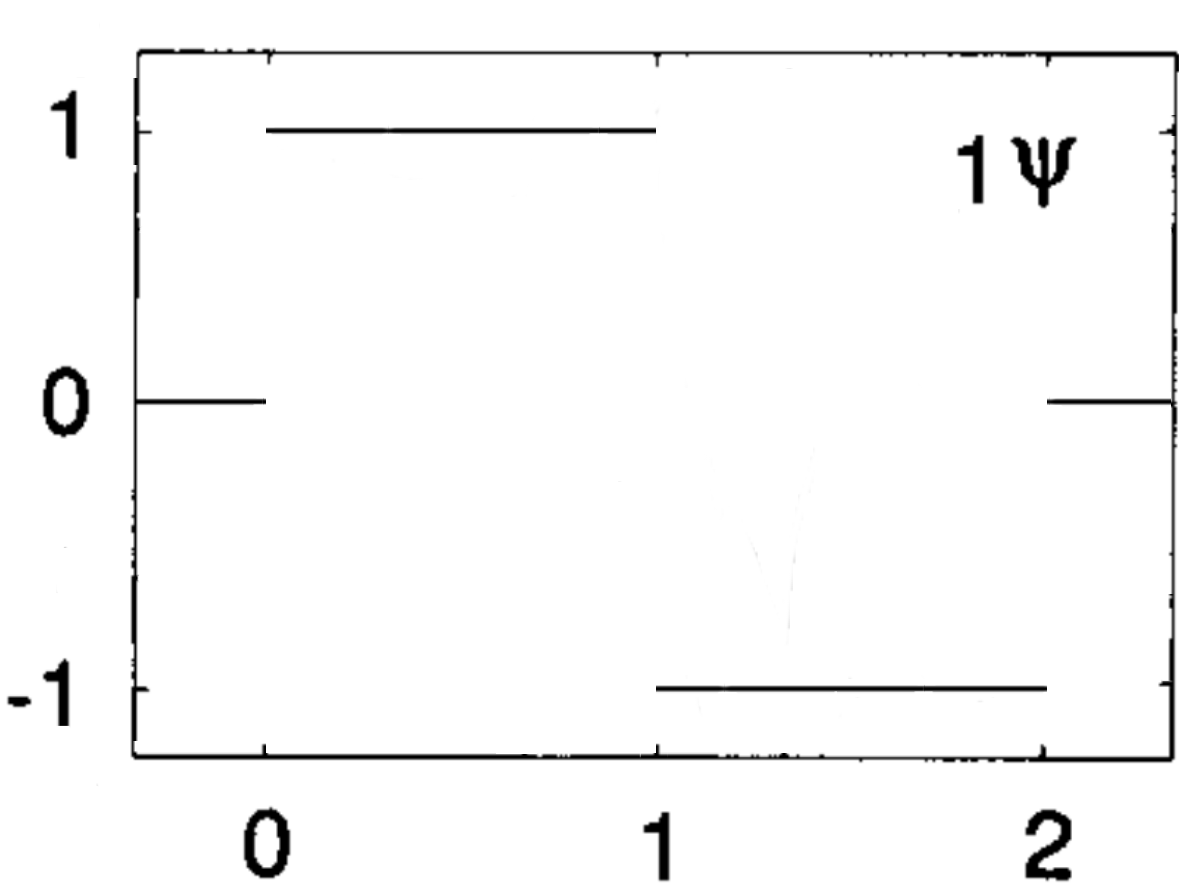
\includegraphics[width=\textwidth]{Figures/Daubechies1}
   \end{subfigure}
   \begin{subfigure}{0.32\textwidth}
   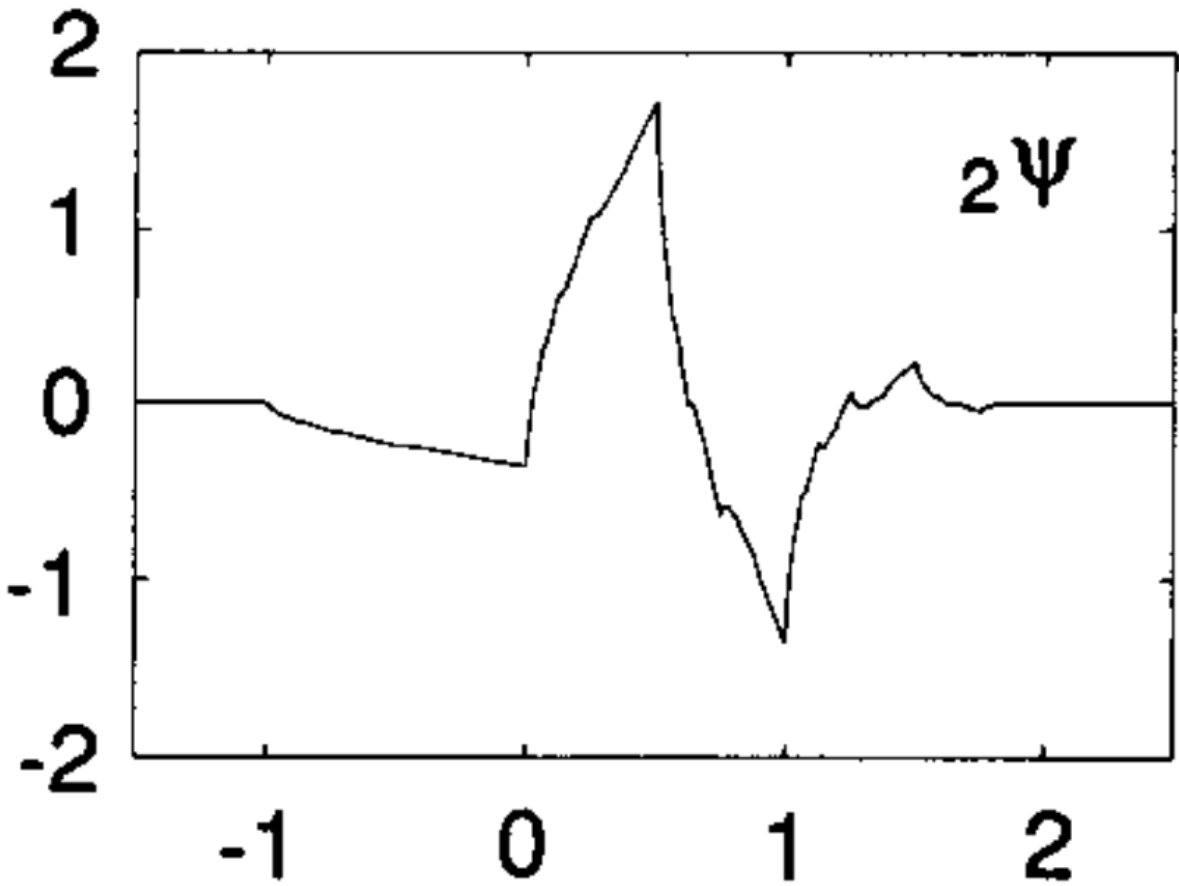
\includegraphics[width=\textwidth]{Figures/Daubechies2}
   \end{subfigure}
   \begin{subfigure}{0.32\textwidth}
   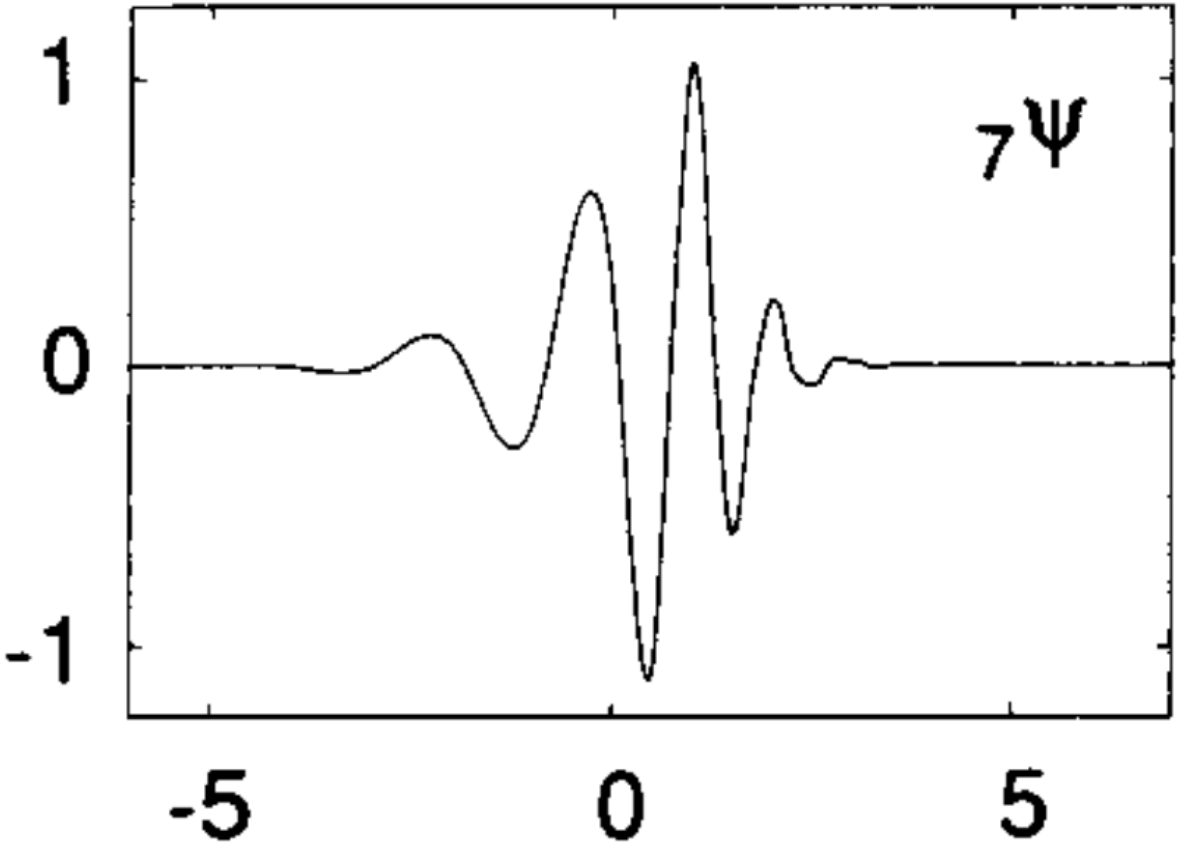
\includegraphics[width=\textwidth]{Figures/Daubechies7}
   \end{subfigure}
   \caption{Daubechies wavelets of the orders 1, 2 and 7 (from left to right) \cite{daubechies}.}
   \label{fig:wavelets}
\end{figure}

Besides their broad use in data compression and analysis, wavelet bases also provide a handy tool to solve partial differential equations and are found to have similar numerical properties as the FEM \cite{FdFeWavelet}.
When applying a wavelet basis to solve a partial differential equation, the weak form (\ref{eq:SEweak}) is used, leading to a similar description as in the FEM scheme \cite{dahlke}.
However, not all wavelets provide a valid basis for partial derivatives since, for example, the Haar-wavelet has a constant derivative of zero and the Daubechies-wavelet $2$ (shown in Figure \ref{fig:wavelets}) is only semi-differentiable at some points \cite{WaveletChem}.
At the same time hand the generality of the wavelet formulation allows to use problem-specific bases that are \textit{e.g.} especially adapted to certain pseudo-differential operators, increasing the convergence properties \cite{dahlke}.
Finding such optimised bases in a systematic way is under current research but one can expect that they could obtain numerically stable, fast and accurate partial derivative solvers \cite{dahlke,kunoth}.
